\documentclass[a4paper, fontsize=11pt]{article}

\usepackage[francais]{babel}
\usepackage[utf8]{inputenc}
\usepackage[T1]{fontenc}
\usepackage{amsmath}
\usepackage{array}
\usepackage{graphicx}
\usepackage{url}

%\setlength{\parindent}{4em}
%\setlength{\parskip}{1em}

\begin{document}

\newcommand{\horrule}[1]{\rule{\linewidth}{#1}} 

\title{
\normalfont \normalsize
\textsc{universite de haute-alsace} \\ [25pt]
\horrule{0.5pt} \\ [0.4cm]
\huge Algorithme de l'Artificial Bee Colony
\horrule{2pt} \\ [0.5cm]
}

\author{Olivier DELIERRE, Ilyasse TISSAFI, Michael GERWILL, Antonin LECLERC}

\maketitle

\normalfont

\section{Introduction}
Dans la nature, différentes espèces vivent en groupe : les bancs de poissons, les nuées d’oiseaux, les troupeaux, les abeilles… Ces dernières sont très bien organisées et très rigoureuses dans leur travail. Des chercheurs se sont donc intéressé au comportement des abeilles pour créer une métaheuristique.

Une métaheuristique est un algorithme d’optimisation permettant de résoudre des problèmes d’optimisation difficile pour lesquels on ne connaît pas de méthode classique plus efficaces. Nous allons donc dans ce rapport parler de l’algorithme ABC (Artificial Bee Colony)\cite{official}.


Dans cet algorithme on distingue trois types d’abeilles : les employées, les éclaireuses et les spectatrices qui ont chacune une tâche bien définie.

\newpage

\tableofcontents

\newpage
%%PAGE 1

\section{L'algorithme}
\subsection{Explication humaine}
L’algorithme simule le comportement d’une colonie d’abeilles, il y a ainsi trois types d’abeilles :
\begin{itemize}
\item Les \textbf{employées} cherchent de la nourriture autour de la source de nourriture qu’elles ont en mémoire et partagent ces informations avec les abeilles spectatrices.
\item Les \textbf{spectatrices}, elles, choisissent les meilleures sources de nourriture parmi celles que les abeilles employées leur ont transmises. 
\item Les \textbf{éclaireuses}, anciennes abeilles employées dont la source de nourriture n’a pas été retenue, cherchent aléatoirement une nouvelle source de nourriture.
\end{itemize}

\subsection{Explication machine}
L'algorithme procède en réalité de la manière suivante :
\begin{enumerate}
\item On commence à générer un nombre défini de solutions, possédant chacune une dimension précisée.
\item Pour chaque étape d'évolution :
\begin{enumerate}
\item On évalue la fitness des différentes solutions
\item Pour chaque solution, on génère une nouvelle solution, et on vérifie si celle-ci est meilleure que la précédente. Si elle l'est, la nouvelle solution remplace l'ancienne. Sinon, un compteur d'essai spécifique à la solution est incrémenté
\item Pour chaque solution, nous décidons aléatoirement, selon la fitness de la solution, si nous lui ré-appliquons la même chose que précédemment.
\item Puis, chaque solution ayant dépassé un nombre d'essais défini est régénéré.
\end{enumerate}
\end{enumerate}

\subsubsection{Formules}
Afin d'arriver à nos fins, certaines formules ont été choisis\cite{wiki} spécialement pour cette algorithme. Les voici :\par
Génération des solutions :
\begin{equation}
x_{mi} = l_i + rand(0,1)*(u_i - l_i)
\end{equation}
\begin{tabular}{@{}>{$}l<{$}l@{}}
l_i & : limite haute du problème\\
u_i & : limite basse du problème\\
\end{tabular}


Génération des nouvelles solutions pour les abeilles employées :
\begin{equation}
\nu_{mi} = x_{mi} + rand(0,1)*(x_{mi} - x_{ki})
\end{equation}
\begin{tabular}{@{}>{$}l<{$}l@{}}
x_k & : une solution aléatoire\\
i & : une dimension aléatoire\\
\end{tabular}

Transformation de la fitness pour calculer une minimisation :
\begin{equation}
fit(\vec{x_m}) = \begin{cases}
	\cfrac{1}{1 + f_m(\vec{x_m})} & \text{si} f_m(\vec{x_m}) >= 0\\
	1 + abs(f_m(\vec{x_m}) & \text{si} f_m(\vec{x_m}) < 0
	\end{cases}
\end{equation}

\newpage

\section{Contraintes}
Voici les différentes contraines qui nous ont été imposées :

\begin{enumerate}
\item Nombre maximum d'exécutions : 30

\item Dimension du problème : 30

\item Nombre d'individus par population : 30

\item Nombre total d'appel de la fonction objectif : $2 \times 10 ^ 3$

\item Nous devions calculer la moyenne ainsi que l'écart type

\item Nous devions comparer nos résultats avec un algorithme de la littérature.
\end{enumerate}

\newpage

\section{Conception de l'algorithme}
\subsection{Les classes}
Cinq classes sont présentes dans le code de cet algorithme. Ceux-ci ont été imposés dans un but de clarté. Les voici :
\begin{enumerate}
\item La classe \textbf{Benchmark} qui contient les différentes fonctions permettant de calculer f(x) de chaque Benchmark.

\item La classe \textbf{SetUpParams} contenant les différents paramètres du problème, défini dans la fonction de démarrage "main".

\item La classe \textbf{Problem} composé des différents éléments représentant un problème (c'est à dire, les bornes haute et basse du problème, sa dimension, ainsi que le code du Benchmark qui sera utilisé).

\item La classe \textbf{Solution} qui contient les valeurs de la solution pour chaque dimension, la fitness, la fitness remaniée (qui permet de générer des probabilités pour les abeilles spectatrices), ainsi que le problème à résoudre.

\item Pour finir, la classe \textbf{MyAlgorithm} qui permet de faire dérouler l'algorithme. Elle contient la totalité des fitness des différentes solutions, les différentes probabilités pour chaque solution d'être choisie, ainsi que le nombre d'essais pour chaque solution.

La principale fonction de cette classe est "\texttt{evolution()}", qui envoie les différentes abeilles en fonction des paramètres qui ont été indiqués.
\end{enumerate} 

\subsection{Schémas}
\begin{figure}[h]
\centering
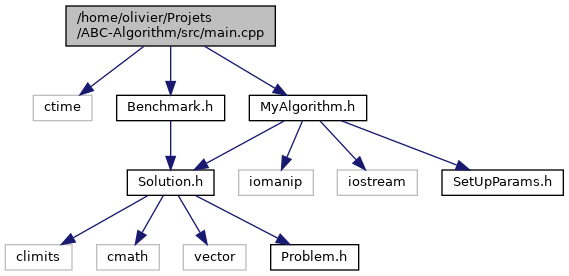
\includegraphics[width=1\textwidth]{diagram.png}
\caption{\label{fig:frog}Diagramme des dépendances des classes.}
\end{figure}

\begin{figure}[h]
\centering
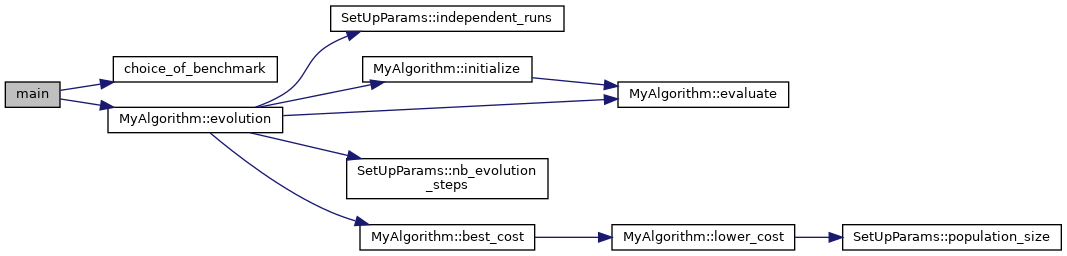
\includegraphics[width=1\textwidth]{callgraph.png}
\caption{\label{fig:frog}Diagramme des appels fonction depuis le main.}
\end{figure}

\clearpage

\newpage

\section{Benchmarks}
Voici les différents Benchmarks qui ont été utilisés afin de vérifier l'efficacité de notre algorithme.
Ceux-ci ont été trouvés à l'aide du site de l'\textbf{Université Simon Fraser du Canada}\cite{sfuca}.

\subsection{Ackley}
\begin{equation}
f(x) = -a \times exp\Bigg(-b \sqrt{\frac{1}{d}\sum_{i=1}^{d} x_i^2}\Bigg) - exp\Bigg(\frac{1}{d}\sum_{i=1}^{d} cos(cx_i)\Bigg) + a + exp(1)
\end{equation}

\begin{figure}[b]
\centering
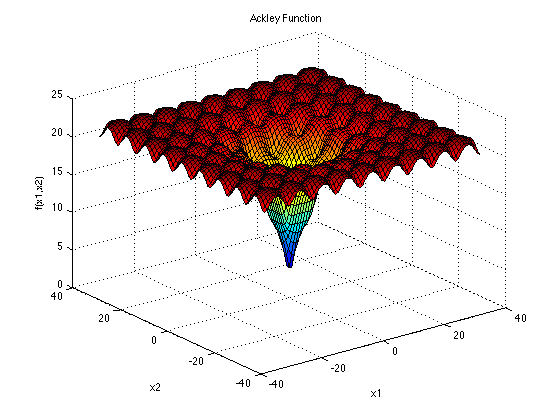
\includegraphics[width=1\textwidth]{ackley.png}
\caption{\label{fig:frog}Fonction d'Ackley.}
\end{figure}

\subsection{Rastrigin}
\begin{equation}
f(x) = 10d + \sum_{i=1}^{d} \big[x_i^2 - 10cos(2 \pi x_i)\big]
\end{equation}

\begin{figure}[b]
\centering
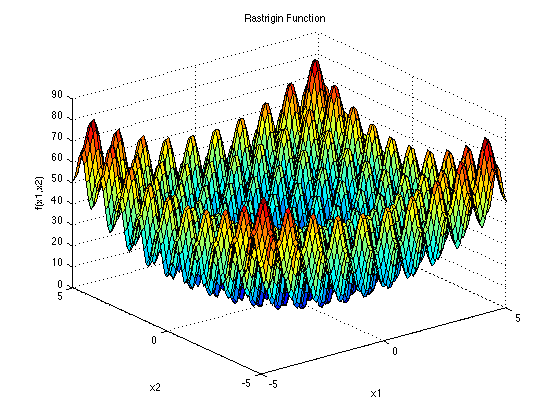
\includegraphics[width=1\textwidth]{rastr.png}
\caption{\label{fig:frog}Fonction de Rastrigin.}
\end{figure}

\subsection{Rosenbrock}
\begin{equation}
f(x) = \sum_{i=1}^{d-1} \big[100(x_{i+1} - x_i^2)^2 + (x_i - 1)^2\big]
\end{equation}

\begin{figure}[b]
\centering
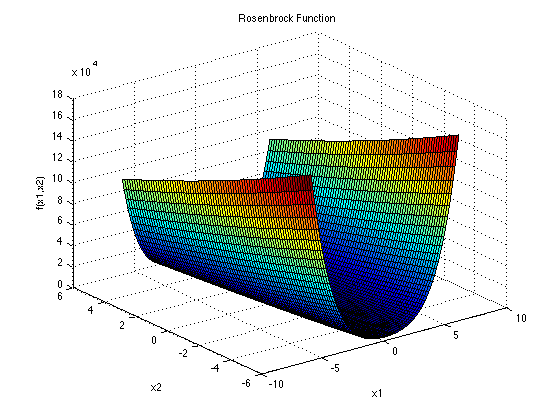
\includegraphics[width=1\textwidth]{rosen.png}
\caption{\label{fig:frog}Fonction de Rosenbrock.}
\end{figure}

\subsection{Schaffer}
\begin{equation}
f(x) = 0.5 + \frac{sin^2(x_1^2 - x_2^2) - 0.5}{[1 + 0.001(x_1^2 + x_2^2)]^2}
\end{equation}

\begin{figure}[b]
\centering
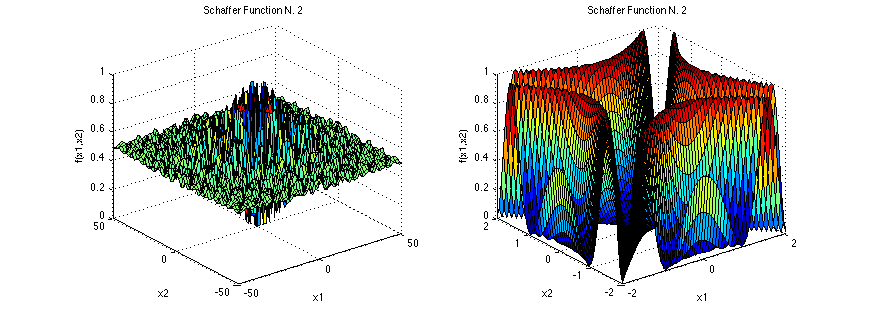
\includegraphics[width=1\textwidth]{schaffer2.png}
\caption{\label{fig:frog}Fonction de Schaffer version 2.}
\end{figure}

\subsection{Schwefel}
\begin{equation}
f(x) = 418.9829d - \sum_{i=1}^{d} x_i sin(\sqrt{|x_i|})
\end{equation}

\begin{figure}[b]
\centering
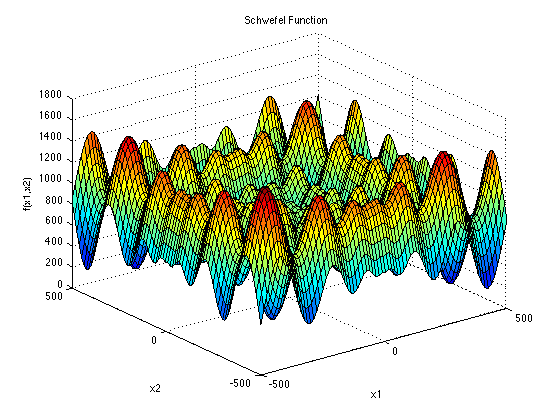
\includegraphics[width=1\textwidth]{schwef.png}
\caption{\label{fig:frog}Fonction de Schwefel.}
\end{figure}

\subsection{Weierstrass}
\begin{equation}
f(x) = \sum_{k=0}^{29} \sum_{n=0}^{20} a^n cos(b^n \pi x_k)
\end{equation}
où $a = 0.5$ et $b = 12$

\begin{figure}[b]
\centering
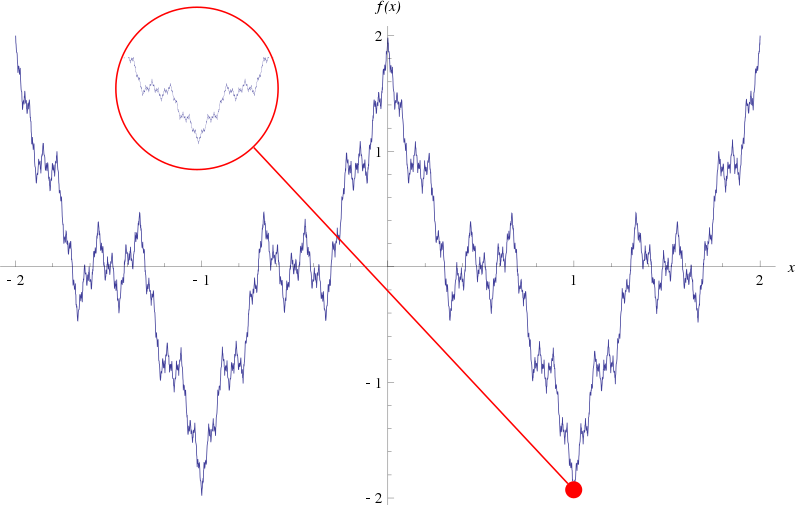
\includegraphics[width=1\textwidth]{weier.png}
\caption{\label{fig:frog}Fonction de Weierstrass.}
\end{figure}

\newpage

\section{Conclusions}
Après réalisation de cet algorithme, la simplicité de celui-ci saute rapidement aux yeux. En plus d'être plutôt performant, celui-ci est plus ou moins simple d'approche pour quelqu'un ayant déjà des connaissances en méta-heuristique.

\subsection{Olivier DELIERRE}
En plus de m'avoir appris énormément de chance sur le réel fonctionnement d'une intelligence artificielle, ce projet m'a permis d'apprendre à travailler en équipe sur un sujet encore inconnu pour nous. Ce fût une expérience intéressante, et très instructive, bien que complexe, au vu des différents problèmes que nous avons pu rencontrer pendant la réalisation de cet algorithme.

\subsection{Ilyasse TISSAFI}
Ce projet portant sur l’intelligence artificielle a été très instructif pour moi, d’une part car l’on a découvert à travers ce projet la science qu’est l’intelligence artificielle, son fonctionnement, son but etc. Et aussi d’autre part car on avait carte blanche afin de mener à bien ce projet. Aussi, l’algorithme ABC, qui est un algorithme très récent a été vraiment intéressant à étudier.

\subsection{Michael GERWILL}
La mission qui nous a été confiée a sûrement été la plus complexe que nous ayons eu à traiter depuis le début de notre cursus universitaire. De plus, le fait que ce projet ait démarré de façon rapide sans réelles connaissances nous a efforcé à réaliser de multiples recherches avant de pouvoir réellement commencer la phase de réalisation. Selon moi, ce projet a été mené à bien notamment grâce à un esprit d'équipe et d'entraide, mais aussi à notre persévérance et à notre détermination sans faille. Nous avons été confrontés à de multiples reprises à des difficultés en terme de compréhension et de conception, donc par ce fait, été contraint de chercher des solutions, d'être autonome ainsi que de se concerter entre membres du groupe pour favoriser au mieux l'aboutissement du projet. En résumé, ce projet aura été l'occasion de découvrir l'intelligence artificielle, ainsi que d'approfondir nos compétences de développement en C++.

\subsection{Antonin LECLERC}

Ce projet a été pour moi une expérience enrichissante car il m’a permis de découvrir l’intelligence
artificiel à travers un problème concret, l’algorithme ABC. Je pense que notre groupe s’est bien
organisé, en effet nous avons commencé par de nombreuses recherches afin de constituer un
document à suivre pour ensuite coder l’algorithme ce qui nous a grandement aidé.
J’ai rencontré des difficultés pour implémenter le code de l’algorithme dans la structure imposée
mais mes collègues ont pu m’éclairer. Je suis satisfait de ce projet car il m’aura permis de progresser
en C++ et dans l’utilisation de GitHub

\newpage

\bibliographystyle{plain}
\bibliography{biblio}

\end{document}
